\documentclass[12pt,a4paper]{report}
\usepackage{fontspec}
\IfFontExistsTF{TeX Gyre Termes}{\setmainfont{TeX Gyre Termes}}{\setmainfont{Liberation Serif}}
\IfFontExistsTF{TeX Gyre Heros}{\setsansfont{TeX Gyre Heros}}{\setsansfont{Liberation Sans}}
\setmonofont[Scale=0.84]{DejaVu Sans Mono}
\usepackage[vietnamese]{babel}
\usepackage[a4paper,margin=1in]{geometry}
\usepackage{amsmath,amssymb,mathtools,bm}
\usepackage{booktabs,tabularx,array,longtable}
\usepackage{graphicx,float}
\usepackage[hidelinks]{hyperref}
\usepackage{fancyhdr,setspace,titlesec,caption,microtype,needspace}
\usepackage{enumitem}
\setstretch{1.15}
\setlength{\parskip}{0.3em}
\setlength{\parindent}{0pt}
\setlength{\headheight}{16pt}
\setcounter{tocdepth}{1}
\setcounter{secnumdepth}{2}
\captionsetup{font=small,labelfont=bf}
\numberwithin{equation}{chapter}
\titleformat{\chapter}[display]{\normalfont\bfseries}{\filleft\Large Chương \thechapter}{0.3em}{\filright\huge}[\vspace{0.4em}\titlerule]
\titlespacing*{\chapter}{0pt}{-10pt}{20pt}
\titleformat{\section}{\large\bfseries}{\thesection}{0.6em}{}
\titleformat{\subsection}{\normalsize\bfseries}{\thesubsection}{0.6em}{}
\pagestyle{fancy}
\fancyhf{}
\lhead{\small CO5177 · Tabular}
\rhead{\small Học kỳ 261 · Tabular}
\cfoot{\thepage}
\fancypagestyle{plain}{\fancyhf{}\lhead{\small CO5177 · Tabular}\rhead{\small Học kỳ 261 · Tabular}\cfoot{\thepage}}
\newcommand{\R}{\mathbb{R}}
\newcommand{\norm}[1]{\left\lVert #1 \right\rVert}
\newcommand{\code}[1]{\texttt{\detokenize{#1}}}
\newcommand{\resultfigure}[3]{\begin{figure}[htbp]\centering\includegraphics[width=#3\textwidth]{generated/figures/#1.png}\caption{#2}\end{figure}}
\hypersetup{pdftitle={CO5177 - Bao cao Tabular},pdfauthor={Huynh Thanh Dat; Luong Minh Duy}}
\emergencystretch=2em

\begin{document}
\hypersetup{pageanchor=false}
\begin{titlepage}\centering
{\large ĐẠI HỌC QUỐC GIA THÀNH PHỐ HỒ CHÍ MINH\par}
{\large\bfseries TRƯỜNG ĐẠI HỌC BÁCH KHOA\par}
{\large KHOA KHOA HỌC VÀ KỸ THUẬT MÁY TÍNH\par}
\vspace{1cm}
\includegraphics[width=3cm]{assets/hcmut-logo.png}\par
\vspace{.8cm}{\large\bfseries NỀN TẢNG LẬP TRÌNH CHO PHÂN TÍCH\par}
{\large\bfseries VÀ TRỰC QUAN DỮ LIỆU\par}{\large Mã môn học: CO5177\par}
\vspace{1cm}\rule{\textwidth}{.6pt}\par\vspace{.4cm}
{\Huge\bfseries BÁO CÁO TABULAR\par}\vspace{.5cm}
{\Large Phân tích và phân loại dữ liệu UCI Adult\par}\vspace{.4cm}\rule{\textwidth}{.6pt}\par
\vspace{.8cm}{\large Học kỳ 261 · Năm học 2026–2027\par}\vspace{.7cm}
\begin{tabular}{ll}Giảng viên: & Lê Thành Sách\\[.5em]
Thành viên: & Huỳnh Thành Đạt · 2570161\\ & Lương Minh Duy · 2570083\end{tabular}
\vfill{\small Thành phố Hồ Chí Minh, tháng 10 năm 2026\par}
\end{titlepage}\hypersetup{pageanchor=true}
\pagenumbering{roman}{\small\tableofcontents}\clearpage\pagenumbering{arabic}

\chapter{Bài toán và dữ liệu}
\section{Mục tiêu}
Bài toán dự đoán nhãn thu nhập lớn hơn 50.000 USD/năm từ các thuộc tính trong UCI Adult.
Phần phân tích tập trung vào dữ liệu thiếu, mã hóa thuộc tính phân loại, chuẩn hóa thuộc tính số
và đánh đổi giữa accuracy với chất lượng dự đoán lớp ít mẫu. Bốn đối chứng gồm dự đoán lớp đa số,
logistic regression, logistic regression cân bằng lớp và histogram gradient boosting.
\section{Nguồn và cấu trúc}
Adult gồm 48.842 bản ghi và 14 thuộc tính từ dữ liệu Census năm 1994, do Barry Becker và Ronny Kohavi cung cấp.
Trang UCI công bố license CC BY 4.0 \cite{adult}. Các thuộc tính số là tuổi, fnlwgt, số năm học,
capital gain, capital loss và số giờ làm mỗi tuần. Tám thuộc tính còn lại là phân loại.
Dấu hỏi được đọc thành giá trị thiếu. Không tạo thiếu nhân tạo.
\section{Chất lượng dữ liệu và chia tập}
Hai tệp official train/test được gộp trước khi tạo một split mới. Nhóm có cùng 14 thuộc tính
nhưng nhãn mâu thuẫn bị loại toàn bộ; nhóm trùng còn lại giữ một bản ghi.
Quy tắc được áp dụng trước khi chia tập, nhằm tránh cùng một vector thuộc tính xuất hiện ở hai phía.
Đây không phải phép đánh giá trên official test gốc, nên điểm số không so trực tiếp với các benchmark dùng split đó.
Loại 10 dòng có nhãn mâu thuẫn và 52 dòng trùng còn lại; giữ 48,780 dòng. Các cột thiếu gồm workclass (2.799), occupation (2.809) và native-country (857).

\begin{figure}[htbp]\centering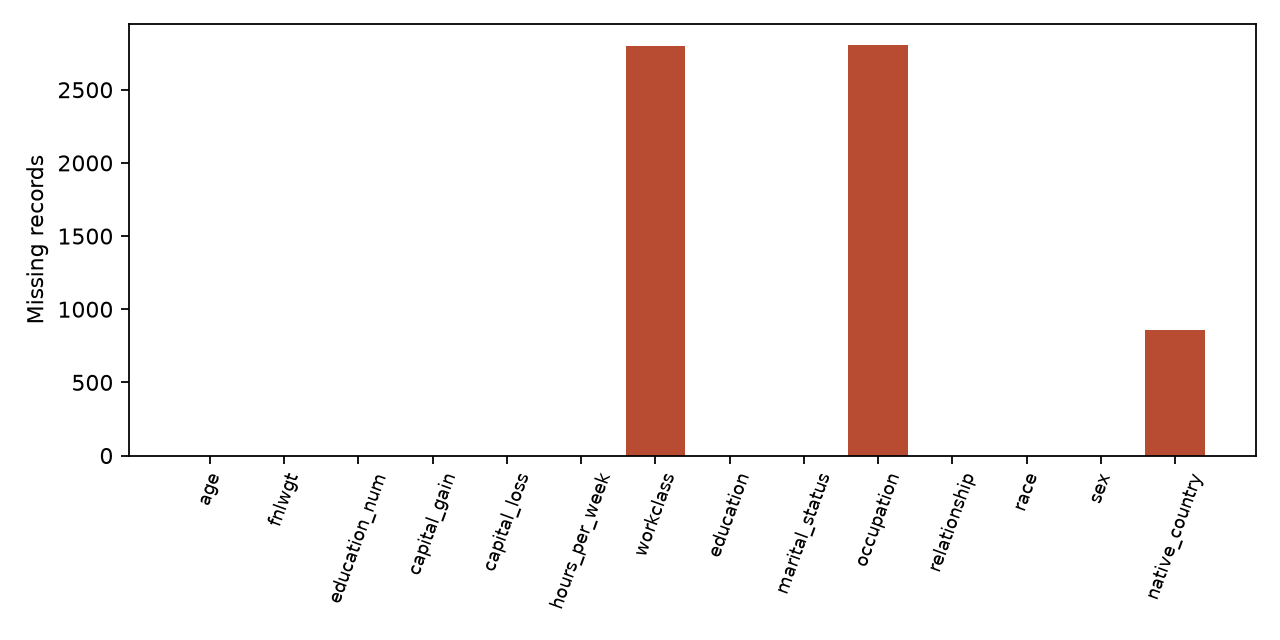
\includegraphics[width=.95\textwidth]{generated/missing.png}
\caption{Giá trị thiếu trong dữ liệu nguồn, trước bước imputation.}\end{figure}
\begin{figure}[htbp]\centering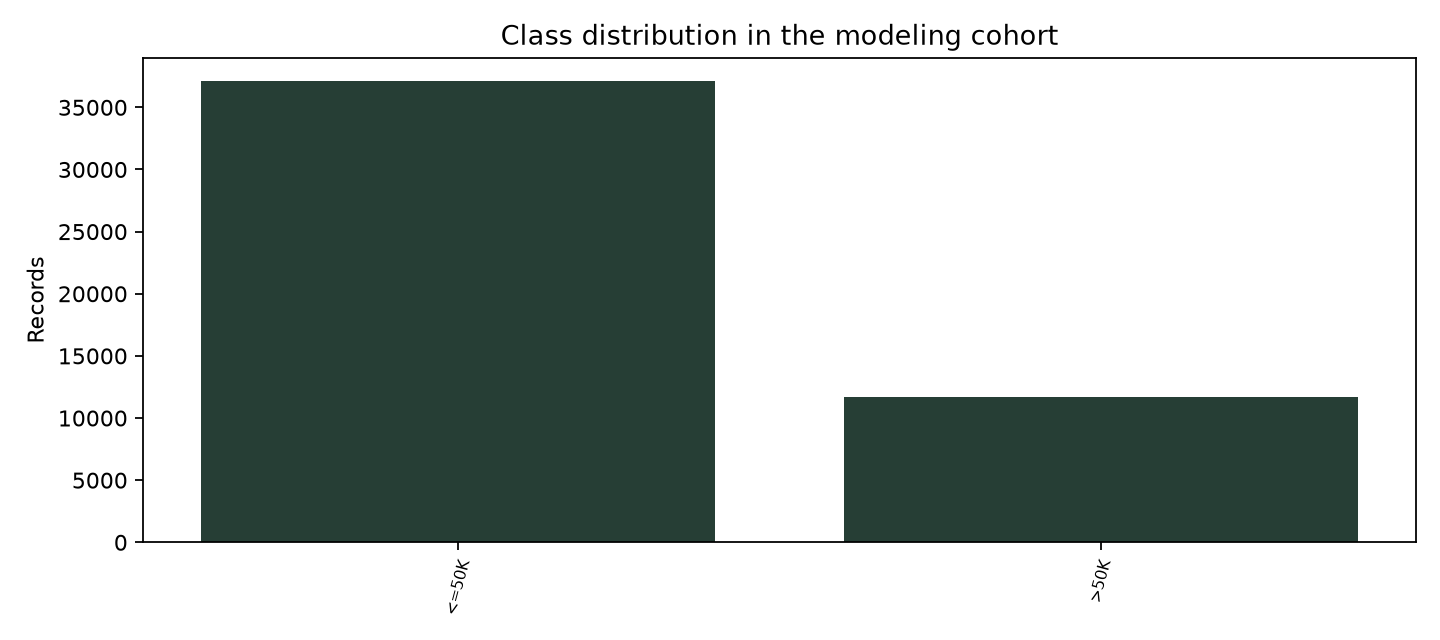
\includegraphics[width=.8\textwidth]{generated/class_counts.png}
\caption{Phân bố hai lớp sau xử lý trùng.}\end{figure}
\chapter{Phương pháp và thiết lập}
\section{Tiền xử lý}
Split phân tầng theo nhãn với tỷ lệ 70/15/15 và seed 2026; phần 30\% còn lại được chia validation/test bằng seed 2027.
Median imputer cho cột số và most-frequent imputer cho cột phân loại chỉ fit trên train.
Logistic regression dùng StandardScaler và one-hot encoding, với lớp mới ở validation/test được bỏ qua trong encoder.
Gradient boosting dùng ordinal encoding cho biến phân loại và khai báo đúng các vị trí categorical;
mã -1 biểu diễn hạng chưa gặp. Không chuẩn hóa các cột số cho cây.
\section{Các mô hình}
Baseline luôn dự đoán lớp phổ biến nhất. Logistic regression thường và bản có class weight balanced
chọn $C\in\{0.1,1,10\}$ theo macro-F1 validation; khi hòa giữ ứng viên xuất hiện trước.
Giới hạn optimizer là 2.000 vòng. Histogram gradient boosting dùng 150 vòng, tối đa 31 lá,
L2 bằng 1 và không early stopping. Các cấu hình cố định trước khi mở test; không refit trên train cộng validation.
\section{Phép đo}
Accuracy, macro-F1, confusion và precision/recall/F1 từng lớp được tính từ prediction test.
Thời gian fit/validation cộng các ứng viên của từng mô hình, không gồm tải dữ liệu và xuất báo cáo.
Chỉ một split và model seed 42 được đo, không báo độ lệch chuẩn hoặc khoảng tin cậy từ một lượt.
Số mẫu train/validation/test là 34,146/7,317/7,317. Indices/ID và chữ ký nguồn được lưu cùng kết quả.

\chapter{Kết quả và phân tích}
\section{So sánh mô hình}
\begin{table}[htbp]\centering\small\setlength{\tabcolsep}{4pt}
\begin{tabularx}{\textwidth}{Xrrrr}\toprule
Mô hình & C & Val F1 & Test acc. & Test F1\\\midrule
Majority baseline & -- & 0.4320 & 76.06\% & 0.4320 \\
Logistic regression & 10.0 & 0.7803 & 85.24\% & 0.7815 \\
Balanced logistic regression & 10.0 & 0.7639 & 81.43\% & 0.7769 \\
Histogram gradient boosting & -- & 0.8147 & 87.48\% & 0.8185 \\
\bottomrule\end{tabularx}
\caption{C được chọn theo validation macro-F1. Test accuracy theo phần trăm; F1 theo thang 0--1.}\end{table}
\begin{figure}[htbp]\centering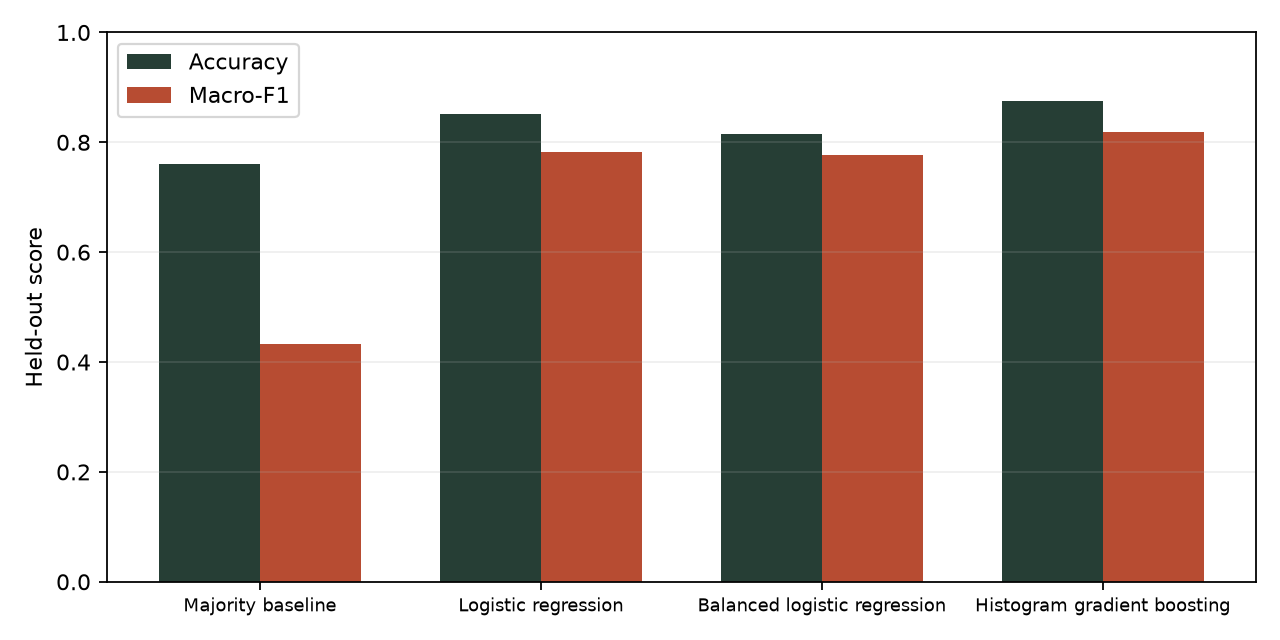
\includegraphics[width=.95\textwidth]{generated/scores.png}
\caption{Accuracy và macro-F1 trên cùng tập test. Không có error bar vì chỉ đo một split/seed.}\end{figure}
\section{Nhận xét}
Gradient boosting đạt accuracy 87.48\% và macro-F1 0.8185, cao hơn logistic regression 2.24 điểm phần trăm accuracy. Cây phân nhánh biểu diễn được các quan hệ phi tuyến và tương tác giữa thuộc tính trong thiết lập này. Đây là diễn giải từ đối chứng đã đo, chưa tách riêng đóng góp từng tương tác.

Cân bằng class weight thay đổi recall lớp >50K từ 0.5908 lên 0.8459, trong khi precision đổi từ 0.7403 xuống 0.5764. Vì vậy, tăng khả năng nhận diện lớp ít mẫu đi kèm nhiều false positive hơn; không thể chỉ đọc accuracy để đánh giá lựa chọn này.

\begin{figure}[htbp]\centering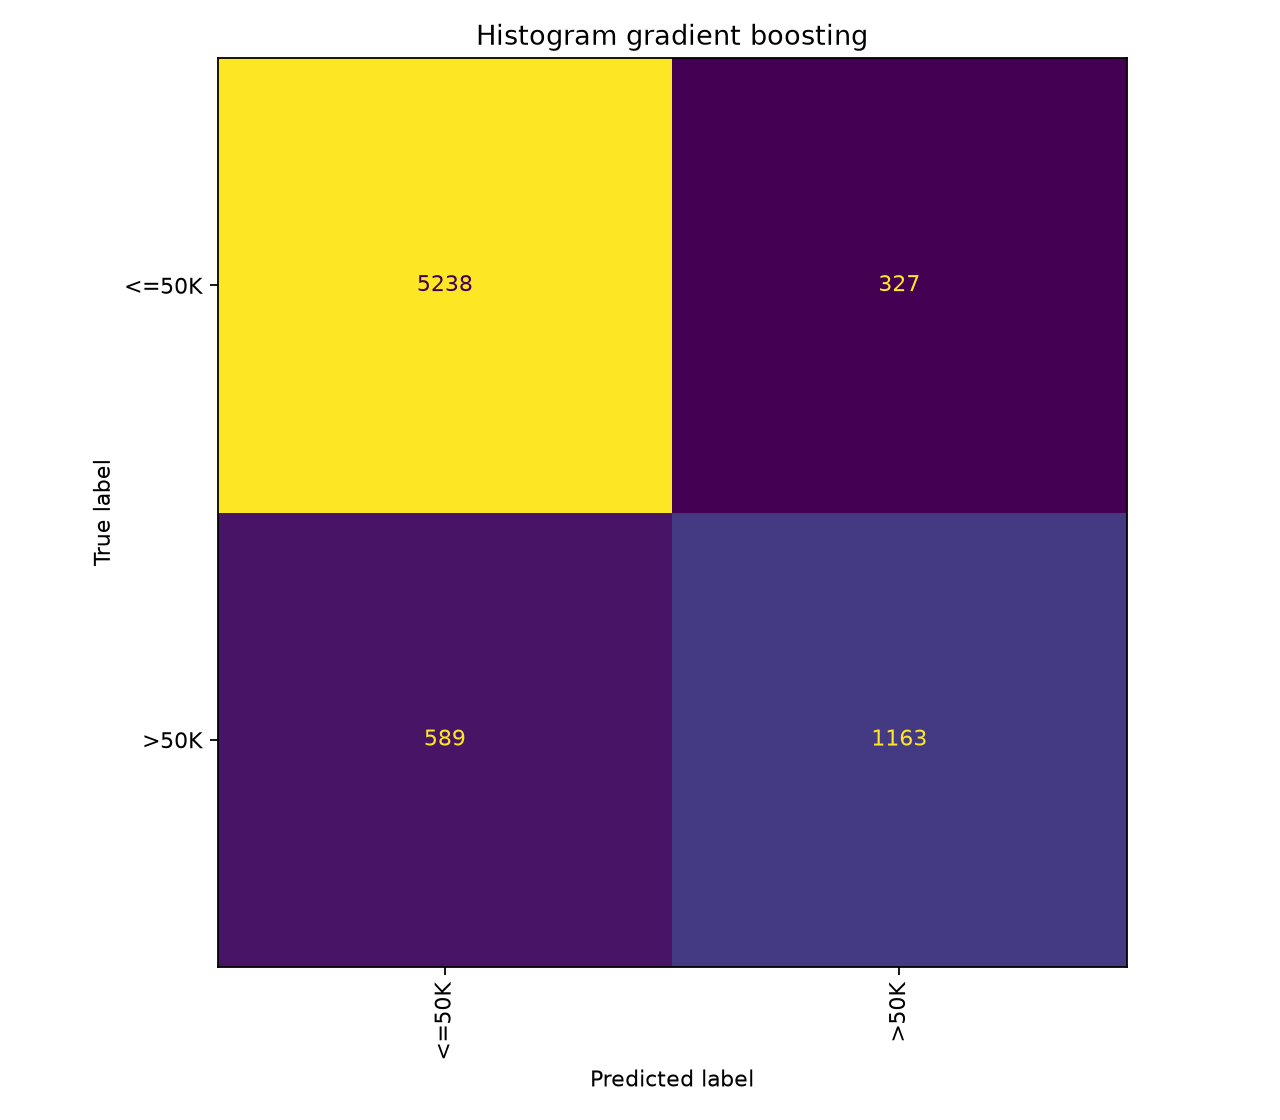
\includegraphics[width=.9\textwidth]{generated/confusion.png}
\caption{Confusion test của mô hình có validation macro-F1 cao nhất; hàng là nhãn thực, cột là dự đoán.}\end{figure}
\chapter{Kết luận và tái lập}
\section{Giới hạn}
Một split và seed chỉ mô tả thiết lập cụ thể; chưa có đánh giá biến thiên hoặc kiểm định thống kê.
Dữ liệu Census lịch sử không đại diện cho thu nhập hiện tại. Đã loại trùng vector thuộc tính nhưng chưa có khóa hộ gia đình
để chia theo nhóm tự nhiên. Fnlwgt được dùng như một feature, không làm sample weight; kết quả không phải ước lượng tỷ lệ dân số.
Chưa khảo sát riêng ảnh hưởng của từng chiến lược imputation hay hiệu quả trên từng nhóm nhân khẩu.
\section{Mã nguồn và lệnh chạy}
Mã nguồn ở \code{src/studies/tabular.py}; cấu hình ở \code{configs/tabular.json}.

\code{python -m studies.tabular} chạy lại toàn bộ thí nghiệm.

Notebook \code{notebooks/tabular.ipynb} thực hiện cùng quy trình.

\code{python -m studies.audit --models} kiểm tra checksum và tính lại chỉ số từ predictions,
đồng thời kiểm tra classifier đã lưu ngoài Git. Chữ ký nguồn/config được kiểm tra không đổi trong lúc đo.
JSON/CSV, split IDs và biểu đồ nằm trong thư mục generated; dữ liệu nguồn, feature cache và model ở data/runs ngoài Git.
Các unit checks kiểm tra loại trùng liên thông, nhãn mâu thuẫn, biến phân loại chưa gặp, thống kê imputer và sửa đổi evidence.

Báo cáo sử dụng AI được đính kèm tại tệp \code{AI_USE_REPORT.md} trong repository.
\begin{thebibliography}{9}\addcontentsline{toc}{chapter}{Tài liệu tham khảo}
\bibitem{adult} B. Becker và R. Kohavi. \emph{Adult}. UCI Machine Learning Repository, 1996. DOI: 10.24432/C5XW20. \url{https://archive.ics.uci.edu/dataset/2/adult}. License CC BY 4.0.
\bibitem{sklearn} Scikit-learn documentation: Pipeline, ColumnTransformer, TfidfVectorizer và classification metrics. \url{https://scikit-learn.org/stable/}.
\end{thebibliography}\end{document}
